\documentclass[]{report}
\usepackage[brazil]{babel}
\usepackage{graphicx} %imagens
\usepackage[hycap]{caption} %legenda
\usepackage[colorlinks=true, allcolors=blue]{hyperref}

% Title Page
\title{Morphoadaequabilitas}
\author{Higor Ribeiro da Costa}


\begin{document}
\maketitle

\begin{abstract}
\end{abstract}

Há muito que me pergunto o porquê de nossas cidades serem tão feias. 'Se temos tanta tecnologia hoje, porque construímos casas, prédios, bairros e cidades assim?' Tenho passado anos com essa dúvida perseguindo meu pensamento e, em parte, é por essa razão que escrevo a presente tese. Posso afirmar com Philippe Daverio que as nossas cidades, sobretudo nossas novas áreas urbanas, são feias.\footnote[1]{Daverio (2022, \textit{s.p.}) fala das periferias da cidades italianas, utilizando-as, eu diria, como um estudo de caso. No fim, ele fala das áreas de expansão urbana, o que, em nosso caso, corresponde a áreas com novos loteamentos, sejam eles contínuos ou contíguos à mancha urbana existente, ou mesmo a novos loteamentos inseridos em vazios urbanos, como glebas remanescentes de um processo de especulação, o que não configura, necessariamente uma periferia. Ademais, o termo 'periferia' costuma evocar a ideia de periferia social, o que, no caso de um traçado urbano, poderia ser materializado por uma favela. Porém, tanto eu quanto Philippe Daverio estamos de acordo que as favelas são 'bonitas', e isso precisamente por seu aspecto morfológico.} Elas suscitam um juízo estético transversal quase que unânime. Talvez 'feiúra' não seja o que melhor define nossas cidades, muito embora \textit{“mentre sul bello si fatica a trovare un parametro congiunto, sul brutto sembra essere meno problematico trovare un terreno comune.”} (DAVERIO, 2022, \textit{s.p.}).\footnote[2]{'Enquanto tem-se dificuldade para encontrar um parâmetro conjunto para [o termo] 'belo', em relação [ao termo] 'feio' parece ser menos problemático encontrar um terreno comum' (tradução nossa).} Desse modo, ao invés de falar em 'feiúra' ou 'beleza', falarei simplesmente de 'harmonia' – tratarei disso no momento oportuno.

Voltemos à retórica pergunta inicial. Penso que, em relação às edificações em geral, temos uma explicação na obra de Gianfranco Caniggia e Gian Luigi Maffei (2008 [1979], pp. 50-57) com dois conceitos fundamentais: \textit{'tipo'} e \textit{'rendimento'}. Basta, por ora, dizer que o \textit{rendimento} é, no caso das edificações, a medida da coerência entre o \textit{tipo} de uma edificação individual e o \textit{tipo} presente nas construções ao seu redor; e que o \textit{tipo} é 'o produto da consciência espontânea radicada no imaginário coletivo, formado pelo universo de elementos físicos ao nosso redor' (COSTA, 2020, p. 43), \textit{i.e.}, o conjunto de características que está presente em cada edificação, ainda que essas edificações não sejam idênticas. Desse modo, quanto mais cada nova edificação '‘se render’ ao \textit{tipo} do ambiente, [assumindo] as características comuns do contexto onde é colocada' (COSTA, 2020, p. 44), maior o seu \textit{rendimento} – e, portanto, maior a harmonia do conjunto. Se isso não resolve a situação em relação às edificações, ao menos a atenua, na medida em que confere maior coesão, e, portanto, harmonia ao conjunto.

Porém, se temos uma solução em relação às edificações – quero dizer, temos ao menos um vislumbre do que fazer –, o mesmo não se dá em relação ao traçado urbano. E aqui faz-se necessário elucidar a diferença entre duas dimensões a que devemos atentar ao analisar essa as cidades. A primeira é a sua '\textit{forma},' aquilo que podemos enxergar diretamente com os olhos e apalpar com mais facilidade na cidade – isto porque a \textit{forma} urbana (\textit{the urban form}) é, por definição, tridimensional, eu diria até 'mais material'. A segunda dimensão é o 'traçado urbano' (\textit{the urban shape}), o 'formato' da \textit{forma,} o contorno que a delineia, o que, por definição, é bidimensional, e, por isso mesmo, 'menos material', ou seja, perceptível pelos sentidos apenas de maneira latente e apenas observável por meio de um processo de abstração que envolve a apreensão da \textit{forma} e sua posterior representação. Representação essa mais esquemática e abstrata do que o seria uma representação direta da \textit{forma} – basta pensar na diferença entre uma pintura, como as de Caspar van Wittel (Figura \ref{fig:popolo}), e um mapa, como o de Giambattista Nolli (Figura \ref{fig:nolli_popolo}).

\begin{figure}[h]
	\centering
	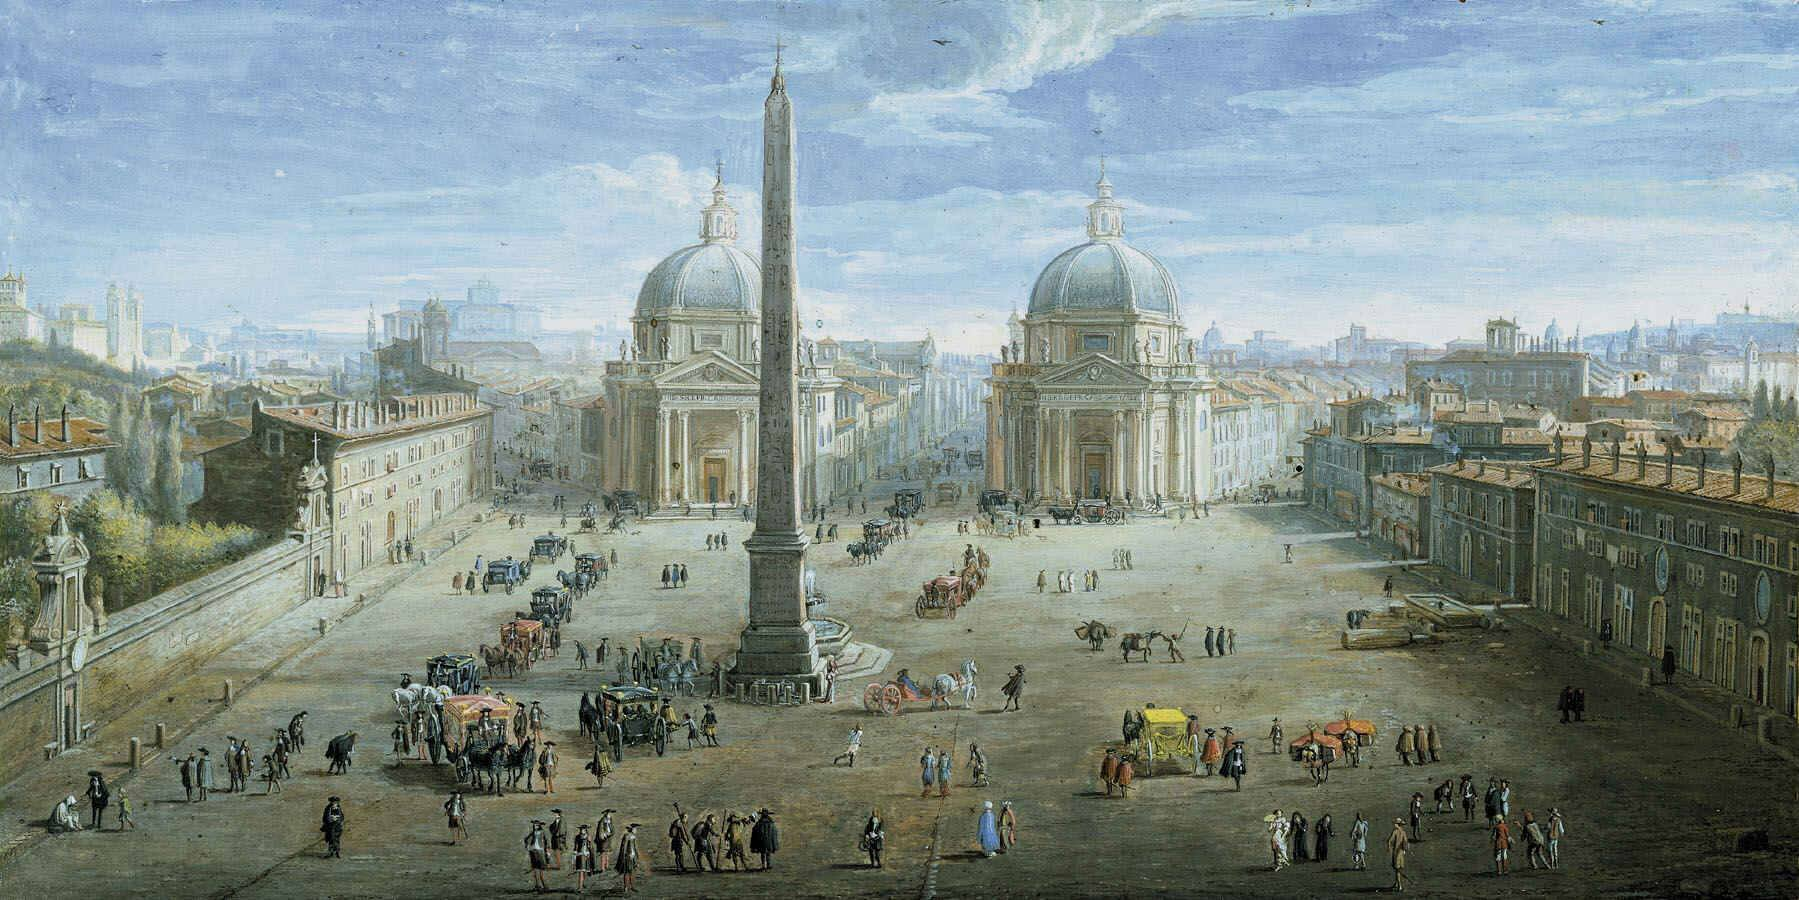
\includegraphics[width=1\textwidth]{/Users/Pancratii/Documents/GitHub/phd/Sections/Projeto_de_Pesquisa_2023-03-18_Teste/Pictures/popolo.jpeg} 
	\captionsetup{labelfont=bf}
	\caption{Vista da \textit{Piazza del Popolo}, em Roma, por Caspar Van Wittel (1652–1736). \textbf{Fonte:} Wikimedia Commons / Sotherby's (coleção privada).}
	\label{fig:popolo}
\end{figure}   

Discorramos rapidamente sobre a ideia de \textit{forma} e traçado. Traçado é o particípio do verbo traçar, \textit{i.e.,} desenhar traços, riscar, sendo o ato ou efeito desse mesmo verbo, resultando, portando, em um 'conjunto de traços', ou, no nosso caso, no 'desenho que representa uma estrutura arquitetônica ou urbanística', o que é equivalente a dizer 'planta', 'projeto', ou, para usar um termo mais antigo, 'traça' (PRIBERAM, TRAÇADO, 2023). Na língua rústica do latim, 'tracto' que dizer 'traçar sulcos', e 'tractus' é a 'delimitação por meio de traços; região, lugar, quarteirão' (FARIA, 1962, p. 1010). Penso que não haja melhor definição que essa: 'delimitação por meio de traços' – que corrobora com a ideia de trajetória de estrada ou linha férrea (PRIBERAM, TRAÇADO, 2023). \textit{Forma,} porém, é um termo mais complexo.

 \begin{figure}
	\centering
	\includegraphics[width=1\textwidth]{/Users/Pancratii/Documents/GitHub/phd/Sections/Projeto_de_Pesquisa_2023-03-18_Teste/Pictures/nolli_popolo.png}
	\captionsetup{labelfont=bf}
	\caption{\textit{La nuova topografia di Roma} (detalhe), de Gianbattista Nolli (1701-1756), com a \textit{Piazza del Popolo} ao norte. \textbf{Fonte:} UC Berkeley Library.}
	\label{fig:nolli_popolo}
\end{figure} 

\textit{Forma} é a 'configuração das coisas na parte exterior', o que é equivalente a 'feitio' e 'formato' (PRIMERAM, FORMA, 2023). No latim, a coisa complica um pouco, com \textit{'forma'} querendo dizer 'fôrma' (que em português é um 'molde sobre o qual ou dentro do qual se coloca alguma substância fluida, que toma o feitio desse molde'), ou 'todo objeto feito na fôrma'; pode, de fato, ser entendida como 'desenho, modelo, planta', mas também pode ser entendida como 'tipo ideal', ou ainda como 'conformação, configuração, constituição' (FARIA, 1962, p. 407). E, se formos para o campo da filosofia, aí é que a confusão aumenta, pois temos um 'sentido filosófico e particularmente metafísico', um 'sentido lógico', outro 'epistemológico', um metodológico', e, por fim, ainda um 'sentido estético' (MORA, 2001b, p. 1126) – e, portanto, a ideia de \textit{'forma'} escapa-nos neste momento.

Desse modo, na presente pesquisa, utilizo o termo 'traçado urbano' para me referir sobremaneira ao desenho das vias (\textit{open spaces}),\footnote[3]{\textit{'The public spaces system of a city includes (...) the open spaces for movement, which we designate, in a simplified way, as streets, (...) [and] also the open spaces for permanence, which we designate as squares and gardens.'} (OLIVEIRA, 2016, p. 17).} ainda que o termo 'traçado urbano' também faça referência aos lotes, quarteirões e contornos edificados (que, não raro, definem o próprio desenho das vias, por meio da conjunção de fachadas).\footnote[4]{Note-se que, diferente do que atualmente é lugar comum, o que definia o que era ou não a rua, seu limite, seu contorno, seu espaço, era precisamente a fachada da edificação, que imprime essa linha ao mesmo tempo imaginária e real no solo, diferente do que ocorre hoje. Hoje, o lugar comum é aquele de que o que define a via é o meio-fio — ou o limite do lote, que não coincide com a implantação da edificação, com a marca que a mesma deixa sobre o solo. E isso é fruto da desvinculação entre edificação e lote, entre os limites da edificação e os limites do lote. Mas, se olharmos para nosso passado urbano, veremos algo bem diferente. Basta olharmos uma pintura de Caspar Van Wittel da \textit{Piazza Navona} em Roma e veremos como a praça já era muitíssimo bem definida (pelas edificações), mesmo sem qualquer indício de calçamento, e muito menos de meio-fio.} Outrossim, quando penso em 'vias', compreendo sua relação com 'nós' urbanos abertos, como praças, e nós urbanos 'cobertos' ou 'fechados', como equipamentos com acesso franqueado ao público, como igrejas, \textit{shoppings} e galerias – desde que com características morfológicas análogas às 'vias' e 'nós' urbanos abertos, o que será elucidado apropriadamente mais adiante.

\end{document}          
